% Options for packages loaded elsewhere
\PassOptionsToPackage{unicode}{hyperref}
\PassOptionsToPackage{hyphens}{url}
%
\documentclass[
  11pt,
  ignorenonframetext,
]{beamer}
\usepackage{pgfpages}
\setbeamertemplate{caption}[numbered]
\setbeamertemplate{caption label separator}{: }
\setbeamercolor{caption name}{fg=normal text.fg}
\beamertemplatenavigationsymbolsempty
% Prevent slide breaks in the middle of a paragraph
\widowpenalties 1 10000
\raggedbottom
\setbeamertemplate{part page}{
  \centering
  \begin{beamercolorbox}[sep=16pt,center]{part title}
    \usebeamerfont{part title}\insertpart\par
  \end{beamercolorbox}
}
\setbeamertemplate{section page}{
  \centering
  \begin{beamercolorbox}[sep=12pt,center]{part title}
    \usebeamerfont{section title}\insertsection\par
  \end{beamercolorbox}
}
\setbeamertemplate{subsection page}{
  \centering
  \begin{beamercolorbox}[sep=8pt,center]{part title}
    \usebeamerfont{subsection title}\insertsubsection\par
  \end{beamercolorbox}
}
\AtBeginPart{
  \frame{\partpage}
}
\AtBeginSection{
  \ifbibliography
  \else
    \frame{\sectionpage}
  \fi
}
\AtBeginSubsection{
  \frame{\subsectionpage}
}
\usepackage{amsmath,amssymb}
\usepackage{lmodern}
\usepackage{iftex}
\ifPDFTeX
  \usepackage[T1]{fontenc}
  \usepackage[utf8]{inputenc}
  \usepackage{textcomp} % provide euro and other symbols
\else % if luatex or xetex
  \usepackage{unicode-math}
  \defaultfontfeatures{Scale=MatchLowercase}
  \defaultfontfeatures[\rmfamily]{Ligatures=TeX,Scale=1}
\fi
\usetheme[]{metropolis}
% Use upquote if available, for straight quotes in verbatim environments
\IfFileExists{upquote.sty}{\usepackage{upquote}}{}
\IfFileExists{microtype.sty}{% use microtype if available
  \usepackage[]{microtype}
  \UseMicrotypeSet[protrusion]{basicmath} % disable protrusion for tt fonts
}{}
\makeatletter
\@ifundefined{KOMAClassName}{% if non-KOMA class
  \IfFileExists{parskip.sty}{%
    \usepackage{parskip}
  }{% else
    \setlength{\parindent}{0pt}
    \setlength{\parskip}{6pt plus 2pt minus 1pt}}
}{% if KOMA class
  \KOMAoptions{parskip=half}}
\makeatother
\usepackage{xcolor}
\newif\ifbibliography
\usepackage{color}
\usepackage{fancyvrb}
\newcommand{\VerbBar}{|}
\newcommand{\VERB}{\Verb[commandchars=\\\{\}]}
\DefineVerbatimEnvironment{Highlighting}{Verbatim}{commandchars=\\\{\}}
% Add ',fontsize=\small' for more characters per line
\newenvironment{Shaded}{}{}
\newcommand{\AlertTok}[1]{\textcolor[rgb]{1.00,0.00,0.00}{\textbf{#1}}}
\newcommand{\AnnotationTok}[1]{\textcolor[rgb]{0.38,0.63,0.69}{\textbf{\textit{#1}}}}
\newcommand{\AttributeTok}[1]{\textcolor[rgb]{0.49,0.56,0.16}{#1}}
\newcommand{\BaseNTok}[1]{\textcolor[rgb]{0.25,0.63,0.44}{#1}}
\newcommand{\BuiltInTok}[1]{#1}
\newcommand{\CharTok}[1]{\textcolor[rgb]{0.25,0.44,0.63}{#1}}
\newcommand{\CommentTok}[1]{\textcolor[rgb]{0.38,0.63,0.69}{\textit{#1}}}
\newcommand{\CommentVarTok}[1]{\textcolor[rgb]{0.38,0.63,0.69}{\textbf{\textit{#1}}}}
\newcommand{\ConstantTok}[1]{\textcolor[rgb]{0.53,0.00,0.00}{#1}}
\newcommand{\ControlFlowTok}[1]{\textcolor[rgb]{0.00,0.44,0.13}{\textbf{#1}}}
\newcommand{\DataTypeTok}[1]{\textcolor[rgb]{0.56,0.13,0.00}{#1}}
\newcommand{\DecValTok}[1]{\textcolor[rgb]{0.25,0.63,0.44}{#1}}
\newcommand{\DocumentationTok}[1]{\textcolor[rgb]{0.73,0.13,0.13}{\textit{#1}}}
\newcommand{\ErrorTok}[1]{\textcolor[rgb]{1.00,0.00,0.00}{\textbf{#1}}}
\newcommand{\ExtensionTok}[1]{#1}
\newcommand{\FloatTok}[1]{\textcolor[rgb]{0.25,0.63,0.44}{#1}}
\newcommand{\FunctionTok}[1]{\textcolor[rgb]{0.02,0.16,0.49}{#1}}
\newcommand{\ImportTok}[1]{#1}
\newcommand{\InformationTok}[1]{\textcolor[rgb]{0.38,0.63,0.69}{\textbf{\textit{#1}}}}
\newcommand{\KeywordTok}[1]{\textcolor[rgb]{0.00,0.44,0.13}{\textbf{#1}}}
\newcommand{\NormalTok}[1]{#1}
\newcommand{\OperatorTok}[1]{\textcolor[rgb]{0.40,0.40,0.40}{#1}}
\newcommand{\OtherTok}[1]{\textcolor[rgb]{0.00,0.44,0.13}{#1}}
\newcommand{\PreprocessorTok}[1]{\textcolor[rgb]{0.74,0.48,0.00}{#1}}
\newcommand{\RegionMarkerTok}[1]{#1}
\newcommand{\SpecialCharTok}[1]{\textcolor[rgb]{0.25,0.44,0.63}{#1}}
\newcommand{\SpecialStringTok}[1]{\textcolor[rgb]{0.73,0.40,0.53}{#1}}
\newcommand{\StringTok}[1]{\textcolor[rgb]{0.25,0.44,0.63}{#1}}
\newcommand{\VariableTok}[1]{\textcolor[rgb]{0.10,0.09,0.49}{#1}}
\newcommand{\VerbatimStringTok}[1]{\textcolor[rgb]{0.25,0.44,0.63}{#1}}
\newcommand{\WarningTok}[1]{\textcolor[rgb]{0.38,0.63,0.69}{\textbf{\textit{#1}}}}
\usepackage{graphicx}
\makeatletter
\def\maxwidth{\ifdim\Gin@nat@width>\linewidth\linewidth\else\Gin@nat@width\fi}
\def\maxheight{\ifdim\Gin@nat@height>\textheight\textheight\else\Gin@nat@height\fi}
\makeatother
% Scale images if necessary, so that they will not overflow the page
% margins by default, and it is still possible to overwrite the defaults
% using explicit options in \includegraphics[width, height, ...]{}
\setkeys{Gin}{width=\maxwidth,height=\maxheight,keepaspectratio}
% Set default figure placement to htbp
\makeatletter
\def\fps@figure{htbp}
\makeatother
\setlength{\emergencystretch}{3em} % prevent overfull lines
\providecommand{\tightlist}{%
  \setlength{\itemsep}{0pt}\setlength{\parskip}{0pt}}
\setcounter{secnumdepth}{-\maxdimen} % remove section numbering
\ifLuaTeX
  \usepackage{selnolig}  % disable illegal ligatures
\fi
\IfFileExists{bookmark.sty}{\usepackage{bookmark}}{\usepackage{hyperref}}
\IfFileExists{xurl.sty}{\usepackage{xurl}}{} % add URL line breaks if available
\urlstyle{same} % disable monospaced font for URLs
\hypersetup{
  pdftitle={Análisis de presencias con procesos de puntos},
  pdfauthor={Gerardo Martín},
  hidelinks,
  pdfcreator={LaTeX via pandoc}}

\title{Análisis de presencias con procesos de puntos}
\subtitle{Tutorial intermedio de spatstat}
\author{Gerardo Martín}
\date{2022-06-29}

\begin{document}
\frame{\titlepage}

\hypertarget{simulaciuxf3n-de-presencias}{%
\section{Simulación de presencias}\label{simulaciuxf3n-de-presencias}}

\begin{frame}{Especificación de un centroide}
\protect\hypertarget{especificaciuxf3n-de-un-centroide}{}
\begin{center}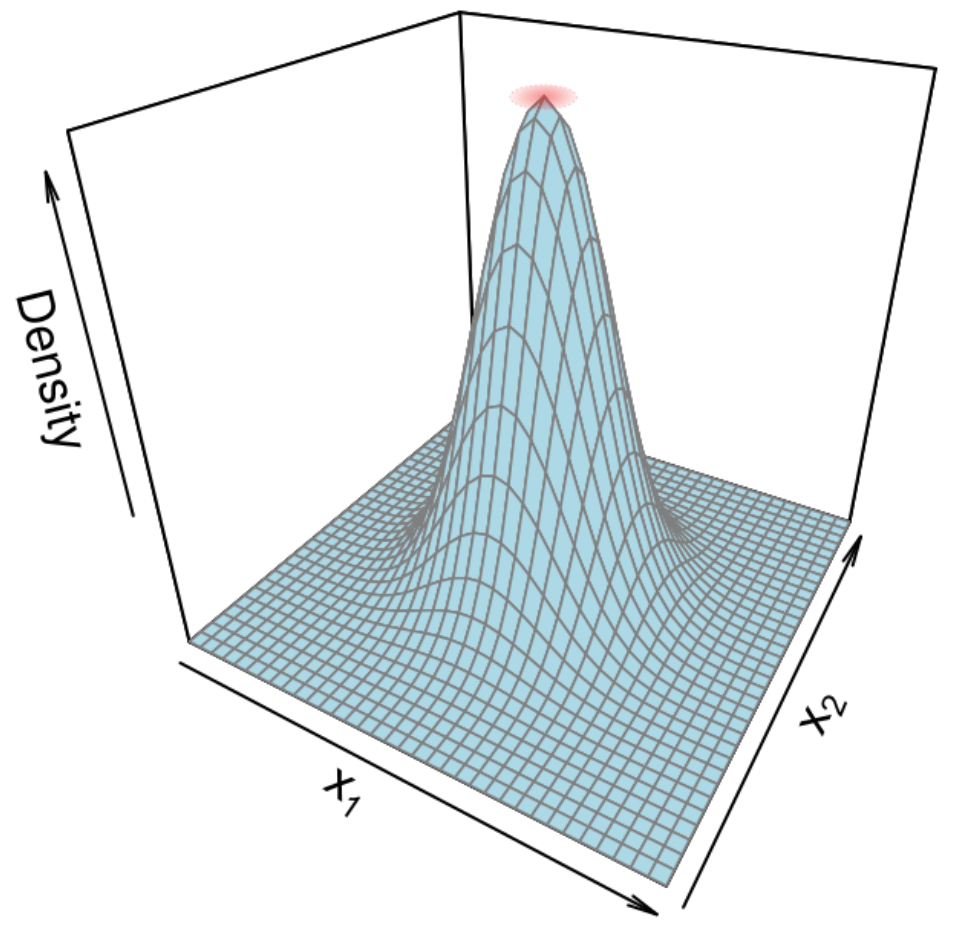
\includegraphics{Figuras/Centroide} \end{center}

\begin{itemize}
\tightlist
\item
  Abundancia alcanza un máximo y disminuye
\item
  Modelos más complicados con varias variables
\end{itemize}
\end{frame}

\begin{frame}[fragile]{Código - generando favorabilidad ``verdadera''}
\protect\hypertarget{cuxf3digo---generando-favorabilidad-verdadera}{}
\begin{Shaded}
\begin{Highlighting}[]
\NormalTok{centroide }\OtherTok{\textless{}{-}} \FunctionTok{cellStats}\NormalTok{(r, mean)}
\NormalTok{r.df }\OtherTok{\textless{}{-}} \FunctionTok{data.frame}\NormalTok{(}\FunctionTok{rasterToPoints}\NormalTok{(r))}
\NormalTok{covar }\OtherTok{\textless{}{-}} \FunctionTok{cov}\NormalTok{(r.df[, }\DecValTok{3}\SpecialCharTok{:}\DecValTok{5}\NormalTok{])}
\NormalTok{md }\OtherTok{\textless{}{-}} \FunctionTok{mahalanobis}\NormalTok{(r.df[, }\DecValTok{3}\SpecialCharTok{:}\DecValTok{5}\NormalTok{], }\AttributeTok{center =}\NormalTok{ centroide, }\AttributeTok{cov =}\NormalTok{ covar)}
\FunctionTok{head}\NormalTok{(md)}
\end{Highlighting}
\end{Shaded}

\begin{verbatim}
## [1] 5.846738 6.383437 6.443874 7.296541 6.475630 6.066614
\end{verbatim}
\end{frame}

\begin{frame}[fragile]{Código - viendo la favorabilidad}
\protect\hypertarget{cuxf3digo---viendo-la-favorabilidad}{}
\begin{Shaded}
\begin{Highlighting}[]
\NormalTok{md.r }\OtherTok{\textless{}{-}} \FunctionTok{rasterFromXYZ}\NormalTok{(}\FunctionTok{data.frame}\NormalTok{(r.df[, }\DecValTok{1}\SpecialCharTok{:}\DecValTok{2}\NormalTok{], md))}
\NormalTok{md.exp }\OtherTok{\textless{}{-}} \FunctionTok{exp}\NormalTok{(}\SpecialCharTok{{-}}\FloatTok{0.5}\SpecialCharTok{*}\NormalTok{md.r)}
\FunctionTok{plot}\NormalTok{(md.exp)}
\end{Highlighting}
\end{Shaded}

\begin{center}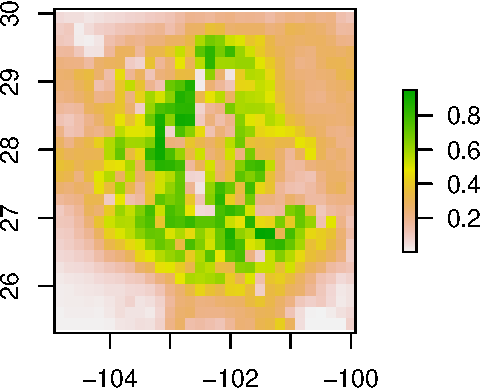
\includegraphics{Tutorial-spatstat-2_files/figure-beamer/unnamed-chunk-4-1} \end{center}
\end{frame}

\begin{frame}[fragile]{Código - simulando los puntos}
\protect\hypertarget{cuxf3digo---simulando-los-puntos}{}
\begin{Shaded}
\begin{Highlighting}[]
\FunctionTok{set.seed}\NormalTok{(}\DecValTok{182}\NormalTok{)}
\NormalTok{puntos}\FloatTok{.2} \OtherTok{\textless{}{-}}\NormalTok{ dismo}\SpecialCharTok{::}\FunctionTok{randomPoints}\NormalTok{(}\AttributeTok{mask =}\NormalTok{ md.exp,}
                                \AttributeTok{n =} \DecValTok{200}\NormalTok{,}
                                \AttributeTok{prob =}\NormalTok{ T)}
\end{Highlighting}
\end{Shaded}

\begin{verbatim}
## Warning in .couldBeLonLat(x, warnings = warnings): CRS is NA. Assuming it is
## longitude/latitude
\end{verbatim}

\begin{Shaded}
\begin{Highlighting}[]
\NormalTok{puntos}\FloatTok{.2} \OtherTok{\textless{}{-}} \FunctionTok{data.frame}\NormalTok{(puntos}\FloatTok{.2}\NormalTok{)}
\NormalTok{puntos}\FloatTok{.2}\SpecialCharTok{$}\NormalTok{x }\OtherTok{\textless{}{-}}\NormalTok{ puntos}\FloatTok{.2}\SpecialCharTok{$}\NormalTok{x }\SpecialCharTok{+} \FunctionTok{rnorm}\NormalTok{(}\DecValTok{200}\NormalTok{, }\DecValTok{0}\NormalTok{, }\FloatTok{0.05}\NormalTok{)}
\NormalTok{puntos}\FloatTok{.2}\SpecialCharTok{$}\NormalTok{y }\OtherTok{\textless{}{-}}\NormalTok{ puntos}\FloatTok{.2}\SpecialCharTok{$}\NormalTok{y }\SpecialCharTok{+} \FunctionTok{rnorm}\NormalTok{(}\DecValTok{200}\NormalTok{, }\DecValTok{0}\NormalTok{, }\FloatTok{0.05}\NormalTok{)}
\end{Highlighting}
\end{Shaded}
\end{frame}

\begin{frame}[fragile]{Código - favorabilidad y puntos}
\protect\hypertarget{cuxf3digo---favorabilidad-y-puntos}{}
\begin{Shaded}
\begin{Highlighting}[]
\FunctionTok{plot}\NormalTok{(md.exp); }\FunctionTok{points}\NormalTok{(puntos}\FloatTok{.2}\NormalTok{)}
\end{Highlighting}
\end{Shaded}

\begin{center}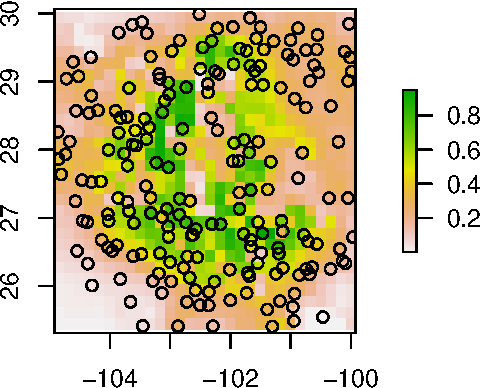
\includegraphics{Tutorial-spatstat-2_files/figure-beamer/unnamed-chunk-6-1} \end{center}
\end{frame}

\hypertarget{formateo-para-spatstat}{%
\section{Formateo para spatstat}\label{formateo-para-spatstat}}

\begin{frame}[fragile]{Cargando las funciones}
\protect\hypertarget{cargando-las-funciones}{}
\begin{Shaded}
\begin{Highlighting}[]
\FunctionTok{source}\NormalTok{(}\StringTok{"Funciones{-}spatstat/imFromStack.R"}\NormalTok{)}
\FunctionTok{source}\NormalTok{(}\StringTok{"Funciones{-}spatstat/winFromRaster.R"}\NormalTok{)}
\FunctionTok{source}\NormalTok{(}\StringTok{"Funciones{-}spatstat/plotQuantIntens.R"}\NormalTok{)}
\end{Highlighting}
\end{Shaded}
\end{frame}

\begin{frame}[fragile]{Formateo rápido}
\protect\hypertarget{formateo-ruxe1pido}{}
\begin{Shaded}
\begin{Highlighting}[]
\NormalTok{r.im }\OtherTok{\textless{}{-}} \FunctionTok{imFromStack}\NormalTok{(r)}
\NormalTok{w }\OtherTok{\textless{}{-}} \FunctionTok{winFromRaster}\NormalTok{(r)}
\NormalTok{puntos.}\FloatTok{2.}\NormalTok{ppp }\OtherTok{\textless{}{-}} \FunctionTok{ppp}\NormalTok{(}\AttributeTok{x =}\NormalTok{ puntos}\FloatTok{.2}\SpecialCharTok{$}\NormalTok{x,}
                  \AttributeTok{y =}\NormalTok{ puntos}\FloatTok{.2}\SpecialCharTok{$}\NormalTok{y,}
                  \AttributeTok{window =}\NormalTok{ w,}
                  \AttributeTok{check =}\NormalTok{ F)}
\NormalTok{Q }\OtherTok{\textless{}{-}} \FunctionTok{pixelquad}\NormalTok{(}\AttributeTok{X =}\NormalTok{ puntos.}\FloatTok{2.}\NormalTok{ppp, }\AttributeTok{W =} \FunctionTok{as.owin}\NormalTok{(w))}
\end{Highlighting}
\end{Shaded}
\end{frame}

\hypertarget{anuxe1lisis-exploratorio}{%
\section{Análisis exploratorio}\label{anuxe1lisis-exploratorio}}

\begin{frame}[fragile]{Autocorrelación}
\protect\hypertarget{autocorrelaciuxf3n}{}
\begin{Shaded}
\begin{Highlighting}[]
\NormalTok{K }\OtherTok{\textless{}{-}} \FunctionTok{envelope}\NormalTok{(puntos.}\FloatTok{2.}\NormalTok{ppp, }\AttributeTok{fun =}\NormalTok{ Kest, }\AttributeTok{nsim =} \DecValTok{39}\NormalTok{)}
\end{Highlighting}
\end{Shaded}

\begin{verbatim}
## Generating 39 simulations of CSR  ...
## 1, 2, 3, 4, 5, 6, 7, 8, 9, 10, 11, 12, 13, 14, 15, 16, 17, 18, 19, 20, 21, 22, 23, 24, 25, 26, 27, 28, 29, 30, 31, 32, 33, 34, 35, 36, 37, 38,  39.
## 
## Done.
\end{verbatim}
\end{frame}

\begin{frame}{Autocorrelación}
\protect\hypertarget{autocorrelaciuxf3n-1}{}
\begin{center}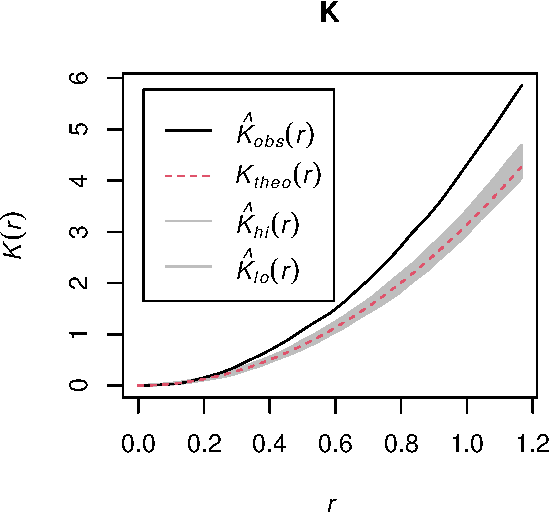
\includegraphics{Tutorial-spatstat-2_files/figure-beamer/unnamed-chunk-10-1} \end{center}
\end{frame}

\begin{frame}{Autocorrelación - notas}
\protect\hypertarget{autocorrelaciuxf3n---notas}{}
\begin{enumerate}
\tightlist
\item
  Pareciera que el proceso está levemente autocorrelacionado
\item
  No sabemos de momento si afectará al modelo
\item
  Debemos poner atención al modelo ajustado
\end{enumerate}
\end{frame}

\begin{frame}[fragile]{Respuestas a variables}
\protect\hypertarget{respuestas-a-variables}{}
\begin{Shaded}
\begin{Highlighting}[]
\FunctionTok{plotQuantIntens}\NormalTok{(}\AttributeTok{imList =}\NormalTok{ r.im,}
                \AttributeTok{noCuts =} \DecValTok{5}\NormalTok{,}
                \AttributeTok{Quad =}\NormalTok{ Q,}
                \AttributeTok{p.pp =}\NormalTok{ puntos.}\FloatTok{2.}\NormalTok{ppp,}
                \AttributeTok{dir =} \StringTok{""}\NormalTok{,}
                \AttributeTok{name =} \StringTok{"Respuestas{-}centroide"}\NormalTok{)}
\end{Highlighting}
\end{Shaded}

\begin{verbatim}
## pdf 
##   2
\end{verbatim}

\href{Respuestas-centroide.pdf}{Ver archivo de gráficas}
\end{frame}

\begin{frame}[fragile]{Consideraciones para proponer modelos}
\protect\hypertarget{consideraciones-para-proponer-modelos}{}
Curvas con forma de campana \(\rightarrow\) fórmula cuadrática

\begin{Shaded}
\begin{Highlighting}[]
\FunctionTok{curve}\NormalTok{(}\FunctionTok{exp}\NormalTok{(}\DecValTok{1} \SpecialCharTok{+}\NormalTok{ x }\SpecialCharTok{{-}}\NormalTok{ x}\SpecialCharTok{\^{}}\DecValTok{2}\NormalTok{), }\AttributeTok{from =} \SpecialCharTok{{-}}\DecValTok{3}\NormalTok{, }\DecValTok{3}\NormalTok{)}
\end{Highlighting}
\end{Shaded}

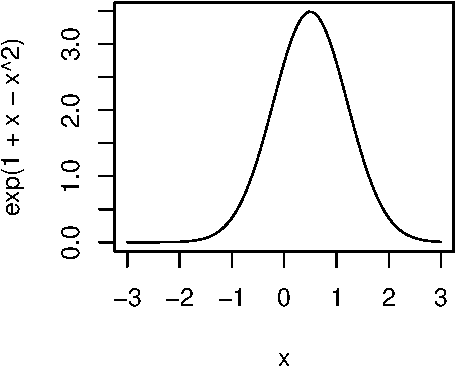
\includegraphics{Tutorial-spatstat-2_files/figure-beamer/unnamed-chunk-12-1.pdf}
\end{frame}

\begin{frame}{Consideraciones para proponer modelos}
\protect\hypertarget{consideraciones-para-proponer-modelos-1}{}
Ecuación lineal:

\[ y = \alpha + \beta_1 x_1 + \dots + \beta_n x_n\] Ecuación polinomial
de 2\(^o\) grado

\[ y = \alpha + \beta_1 x_1 + \beta_1' x_1^2 + \dots + \beta_n x_n + \beta_n' x_n^2\]
Recordemos que \(y = \log \lambda\)
\end{frame}

\begin{frame}[fragile]{¿Qué variables podemos incluir en el mismo
modelo?}
\protect\hypertarget{quuxe9-variables-podemos-incluir-en-el-mismo-modelo}{}
\textbf{Regla de oro}: Aquellas que no estén correlacionadas

\begin{itemize}
\tightlist
\item
  Que \(x_1\) no sea predictor de \(x_2\)
\item
  No se puede atribuir efecto de \(x_1\) ó \(x_2\) sobre \(\lambda\)
\item
  Necesitamos medir correlación entre pares de variables
  (\texttt{pairs})
\end{itemize}
\end{frame}

\begin{frame}[fragile]{Medición de correlación entre covariables}
\protect\hypertarget{mediciuxf3n-de-correlaciuxf3n-entre-covariables}{}
\begin{Shaded}
\begin{Highlighting}[]
\FunctionTok{pairs}\NormalTok{(r)}
\end{Highlighting}
\end{Shaded}

\begin{center}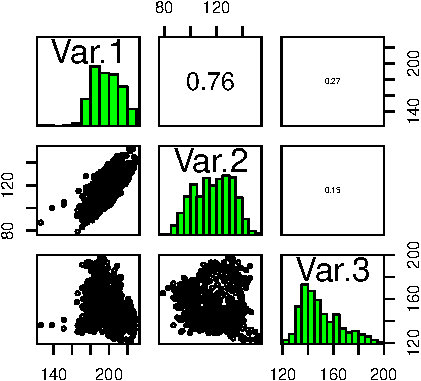
\includegraphics{Tutorial-spatstat-2_files/figure-beamer/unnamed-chunk-13-1} \end{center}
\end{frame}

\end{document}
